\documentclass[10pt]{beamer}

\usepackage[utf8]{inputenc}
\usepackage{tcolorbox}
\usepackage{tikz}
\usepackage{tikz-3dplot}
\usetikzlibrary{intersections,calc,,angles,quotes,through}
\usepackage{amsmath}
\usepackage{graphicx}
\usepackage{cases}
\def \heart {\textcolor{blue}{$\heartsuit$} }
\def \C {\mathcal{C}}
\def \orthog {\underline{\perp}}
\def\arcos{\operatorname{arcos}}

\newcommand{\vect}[1] {
  \overrightarrow{#1}}

\tcbset{%
	basic/.style={colframe=black,
		      colback=white,
		      top= 0mm,
		      bottom = 2mm,
		      boxsep=0mm
		      }
}
\tikzset{
    invisible/.style={opacity=0},
    visible on/.style={alt={#1{}{invisible}}},
    alt/.code args={<#1>#2#3}{%
      \alt<#1>{\pgfkeysalso{#2}}{\pgfkeysalso{#3}} % \pgfkeysalso doesn't change the path
    },
  }

    
\begin{document}  
    \beamertemplatenavigationsymbolsempty
    \setlength{\abovedisplayskip}{0pt}
    \setlength{\belowdisplayskip}{0pt}
    \frame{
	  
	  \frametitle{Q3 Juillet 2003.}
	  %\renewcommand{\theenumi}{\alph{enumi})}
	  On considère un quadrilatère convexe $ABCD$. On note $E$ le milieu de $[A, C]$ et $F$
	  le milieu de $[B, D]$. Démontrer que \\ \medskip
	  
	  $|\vect{AB}|^2 + |\vect{BC}|^2 + |\vect{CD}|^2 + |\vect{DA}|^2 = |\vect{AC}|^2 + |\vect{BD}|^2 + 4|\vect{EF}|^2$.
	  \vfill
	  
	  \pause
	  % hypothèses et thèse
	  \begin{tcolorbox}[basic] 
	      \begin{columns}[t]
		 
		 \column{.5\textwidth}\centering
		      
		      \underline{Hypothèses} 
		      \begin{itemize}
		      \item $|AE|=|EC|$,
		      \item $|BF|=|FD|$.
		      \end{itemize}

		  
		  \column{.5\textwidth}\centering
		      
		      \underline{Thèse} \\
		      \smallskip
		      $|\vect{AB}|^2 + |\vect{BC}|^2 + |\vect{CD}|^2 + |\vect{DA}|^2$ \\ \medskip
		      $= |\vect{AC}|^2 + |\vect{BD}|^2 + 4|\vect{EF}|^2$.
		
	      \end{columns}
	  \end{tcolorbox}
    }

    \frame{ 
	  % résolution ex1
	  \begin{columns}[t]
		\column{.5\textwidth}\centering 
		

			\underline{Dessin}\\
			
				  \begin{figure}[h]
				  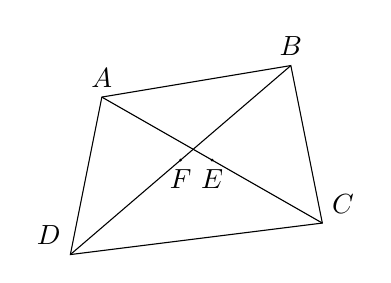
\begin{tikzpicture}[scale=0.8]
			          %projection ($(X)!(B')!(B)$)
			          %nommer chemin 'name path
			          %intersection \path [name intersections={of=d and gb,by=G}];
			          %animation  \draw[visible on=<1>] 
				  %           \draw[visible on=<{2,4}>]
				  %angle arc[radius = 6mm, start angle= 180, end angle= 225] node [below left,pos=0.3]{$\alpha$}
				  %angle \pic [draw,"$\alpha$", angle eccentricity=1.5] {angle = A'--A--B};
				  %perpendiculaire ($(A')!3cm!-90:(A)$)
				  %QUADRILATERE
				  \coordinate[label=above:$A$](A) at (-1.5,1);
				  \coordinate[label=above:$B$](B) at (1.5,1.5);
				  \coordinate[label=above right:$C$](C) at (2,-1);
				  \coordinate[label=above left:$D$](D) at (-2,-1.5);
				  \draw (A)-- (B) -- (C) -- (D) --cycle;
				  %E
				  \draw (A) -- coordinate[label=below:$E$](E) (C);
				  \fill (E) circle (0.025);
				  %F
				  \draw (B) -- coordinate[label=below:$F$](F) (D);
				  \fill (F) circle (0.025);
				  \end{tikzpicture}
				  \end{figure}
			
				  \begin{tcolorbox}[basic] 
				      
				    \smallskip
				    \underline{Hypothèses} 
				    \begin{enumerate}
				    \item $|AE|=|EC|$,
				    \item $|BF|=|FD|$.
				    \end{enumerate}
							      
				    \underline{Thèse} \\
				    \smallskip
				    $|\vect{AB}|^2 + |\vect{BC}|^2 + |\vect{CD}|^2 + |\vect{DA}|^2$ \\ \medskip
				    $= |\vect{AC}|^2 + |\vect{BD}|^2 + 4|\vect{EF}|^2$.
				    \end{tcolorbox}
		
		
		\column{.51\textwidth}\centering
		
		\underline{Résolution}\\ \flushleft
		
		\begin{align*}
		\vect{AC}=&\vect{AB} + \vect{BC}, \\[0.5em]
		\vect{BD}=&\vect{BC} + \vect{CD}, \\[0.5em]
		\vect{EF}=&\vect{EA} + \vect{AD} + \vect{DF} \\
				   =&\frac{\vect{CA}}{2} + \vect{AD} + \frac{\vect{DB}}{2} \\
				   =&\frac{\vect{CB}+\vect{BA}}{2} + \vect{AD} + \frac{\vect{DA}+\vect{AB}}{2} \\
				   =&\frac{\vect{AD}}{2}-\frac{\vect{BC}}{2}. \\[0.5em]
	        \end{align*}
	        
	        \vspace{-5mm}
	        
		\heart Le produit scalaire est commutatif et distributif. \\ \medskip
		
		\vspace{-4mm}
		
		\begin{align*}
	    |\vect{AC}|^2=&\vect{AC}\cdot\vect{AC}, \\
			 =&|\vect{AB}|^2 + 2\vect{AB}\cdot\vect{BC} + |\vect{BC}|^2.
		\end{align*}
 
	   \end{columns}
    
    
    
    }
	  
  
  \frame{
  Thèse : $|\vect{AB}|^2 + |\vect{BC}|^2 + |\vect{CD}|^2 + |\vect{DA}|^2
				    = |\vect{AC}|^2 + |\vect{BD}|^2 + 4|\vect{EF}|^2$. \\ \bigskip
  \begin{align*}
   &|\vect{AC}|^2 + |\vect{BD}|^2 + 4|\vect{EF}|^2, \\[0.5em]
  =&|\vect{AB}|^2+3|\vect{BC}|^2+|\vect{CD}|^2+|\vect{AD}|^2 + 2(\vect{BC}\cdot\vect{CD} -
						      \vect{BC}\cdot\vect{AD} + \vect{BC}\cdot\vect{AB}), \\[0.5em]
  =&|\vect{AB}|^2+3|\vect{BC}|^2+|\vect{CD}|^2+|\vect{AD}|^2 + 2\vect{BC}\cdot( \vect{CD} + \vect{DA} + \vect{AB}), \\[0.5em]
  =&|\vect{AB}|^2+3|\vect{BC}|^2+|\vect{CD}|^2+|\vect{AD}|^2 + 2\vect{BC}\cdot\vect{CB}, \\[0.5em]  
  =&|\vect{AB}|^2+|\vect{BC}|^2+|\vect{CD}|^2+|\vect{AD}|^2. \\ 
  \end{align*} \hfill $\qed$
  


  
  
  
  }
\end{document}
